% ============================================================================
\section{Modern ASR}
% ============================================================================

% --- Stanford CS224S lec11, slides 4--37: Conformer, Whisper, deployment ---
\begin{frame}{Modern ASR: Conformer and Whisper}
  \begin{itemize}
    \item After CTC/RNN-T hybrids, \textbf{Conformer} encoders and \textbf{Whisper}-scale weak supervision define current practice.
  \end{itemize}
\end{frame}

% --- Stanford CS224S lec11, slide 4 ---
% \begin{frame}{Conformer: Convolution-augmented Transformer for Speech Recognition}
%   A conformer is a transformer encoder with a convolutional module in the transformer layer
%   \centering
%   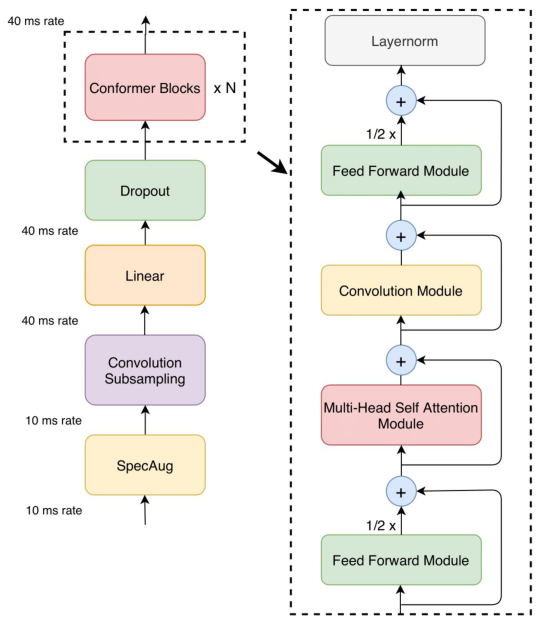
\includegraphics[width=\textwidth,height=0.92\textheight,keepaspectratio]{assets/New-Lecture-STT/cs224s_lec11_slide_04.png}
% \end{frame}

\begin{frame}{Conformer: Convolution-augmented Transformer for Speech Recognition}
  \begin{itemize}\footnotesize
    \item Sequence-to-sequence transformer with multi-headed self attention.
    \item Combines attention (global context) with convolution (local invariance).
    \item Uses RNN-T loss architecture.
  \end{itemize}
  \vspace{0.6em}
  \centering
  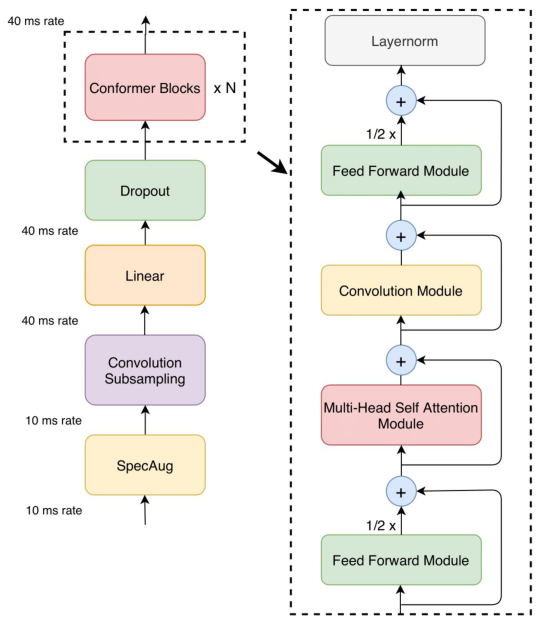
\includegraphics[width=\textwidth,height=0.82\textheight,keepaspectratio]{assets/New-Lecture-STT/cs224s_lec11_slide_04.png}

  \vspace{0.6em}
  {\scriptsize
  \textbf{Figure:} Conformer encoder model architecture.
  Comprises two macaron-like feed-forward layers with half-step residual connections sandwiching the multi-headed self-attention and convolution modules.
  This is followed by a post layernorm.
  \textit{(Gulati et al., 2020)}
  }
\end{frame}

% --- Stanford CS224S lec11, slide 5 ---
\begin{frame}{SpecAugment: Augmenting data to increase dataset size}
  \begin{itemize}
    \item Mask time/frequency bands in log-mel during training for robustness.
  \end{itemize}
  \centering
  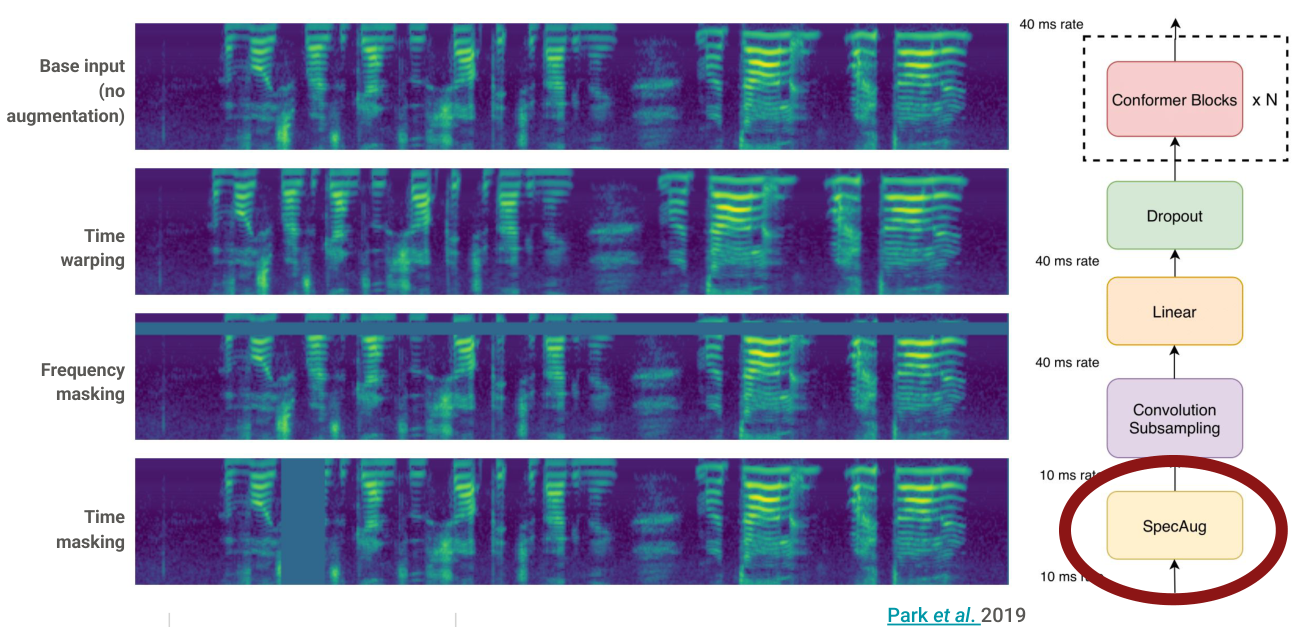
\includegraphics[width=\textwidth,height=0.82\textheight,keepaspectratio]{assets/New-Lecture-STT/cs224s_lec11_slide_05.png}
\end{frame}

% --- Stanford CS224S lec11, slide 6 ---
\begin{frame}{Convolution subsampling: Log mel spectrogram is an image}
  \centering
  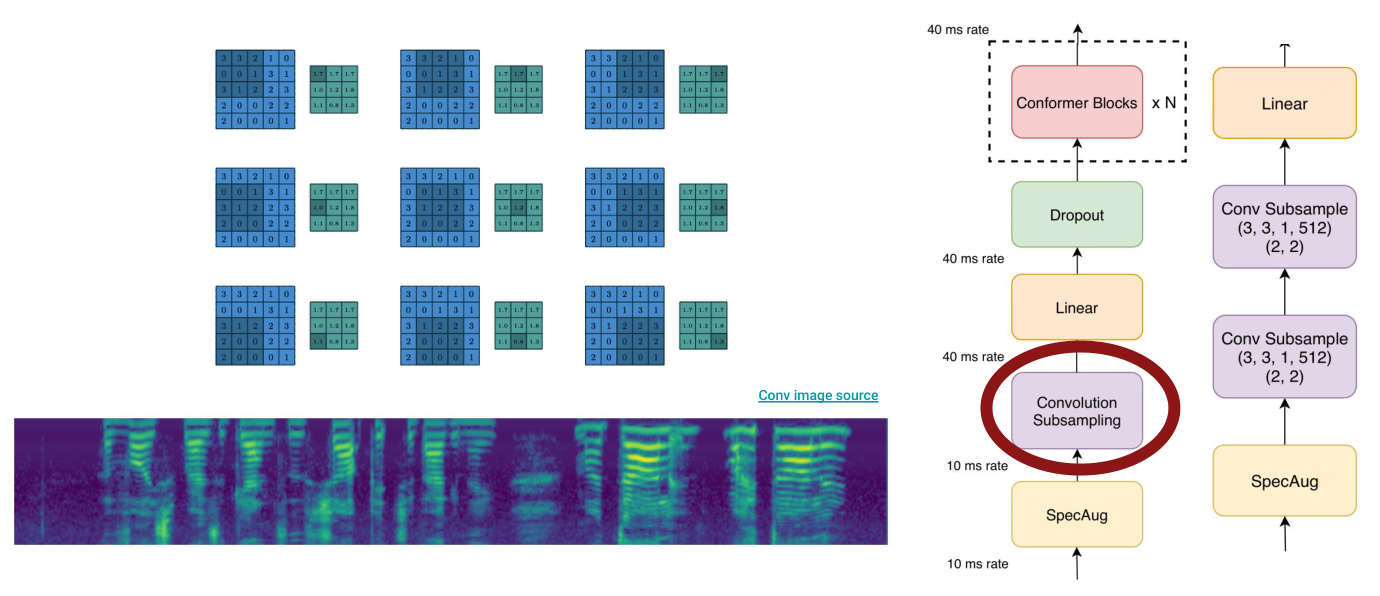
\includegraphics[width=\textwidth,height=0.92\textheight,keepaspectratio]{assets/New-Lecture-STT/cs224s_lec11_slide_06.png}
\end{frame}


% --- Stanford CS224S lec11, slide 9 ---
% \begin{frame}{Transformer encoder to conformer encoder}
%   A conformer is a transformer encoder with a convolutional module in the transformer layer
%   \centering
%   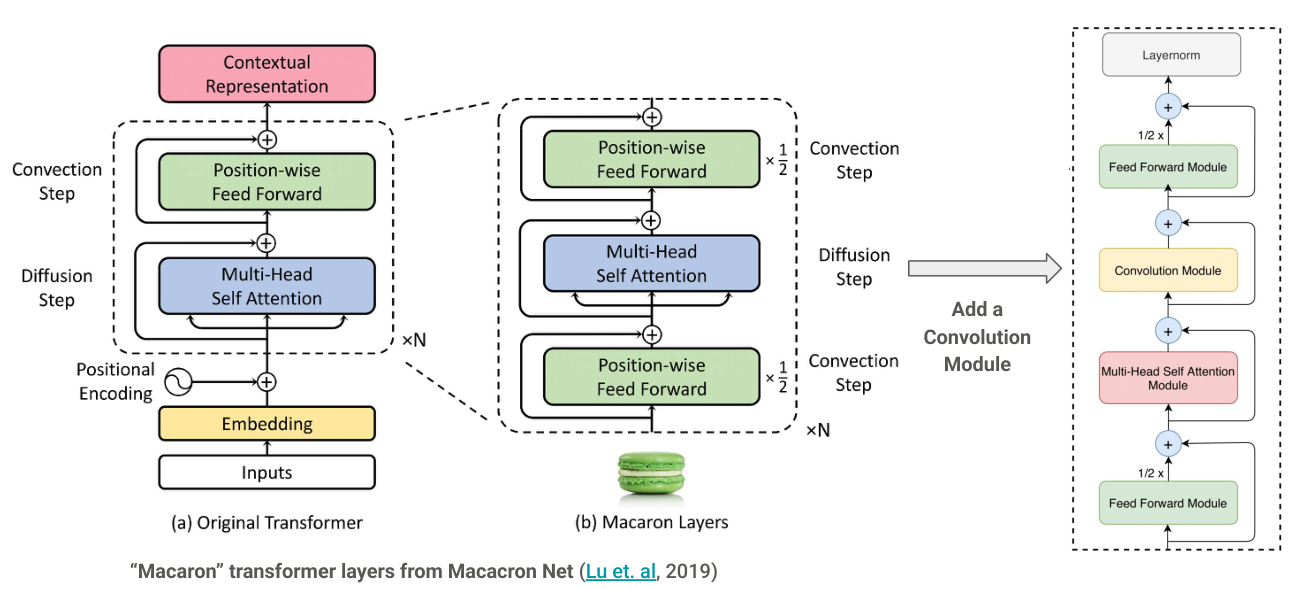
\includegraphics[width=\textwidth,height=0.92\textheight,keepaspectratio]{assets/New-Lecture-STT/cs224s_lec11_slide_09.png}
% \end{frame}

% --- Stanford CS224S lec11, slide 11 ---
% \begin{frame}{Conformer architecture overview}
%   \centering
%   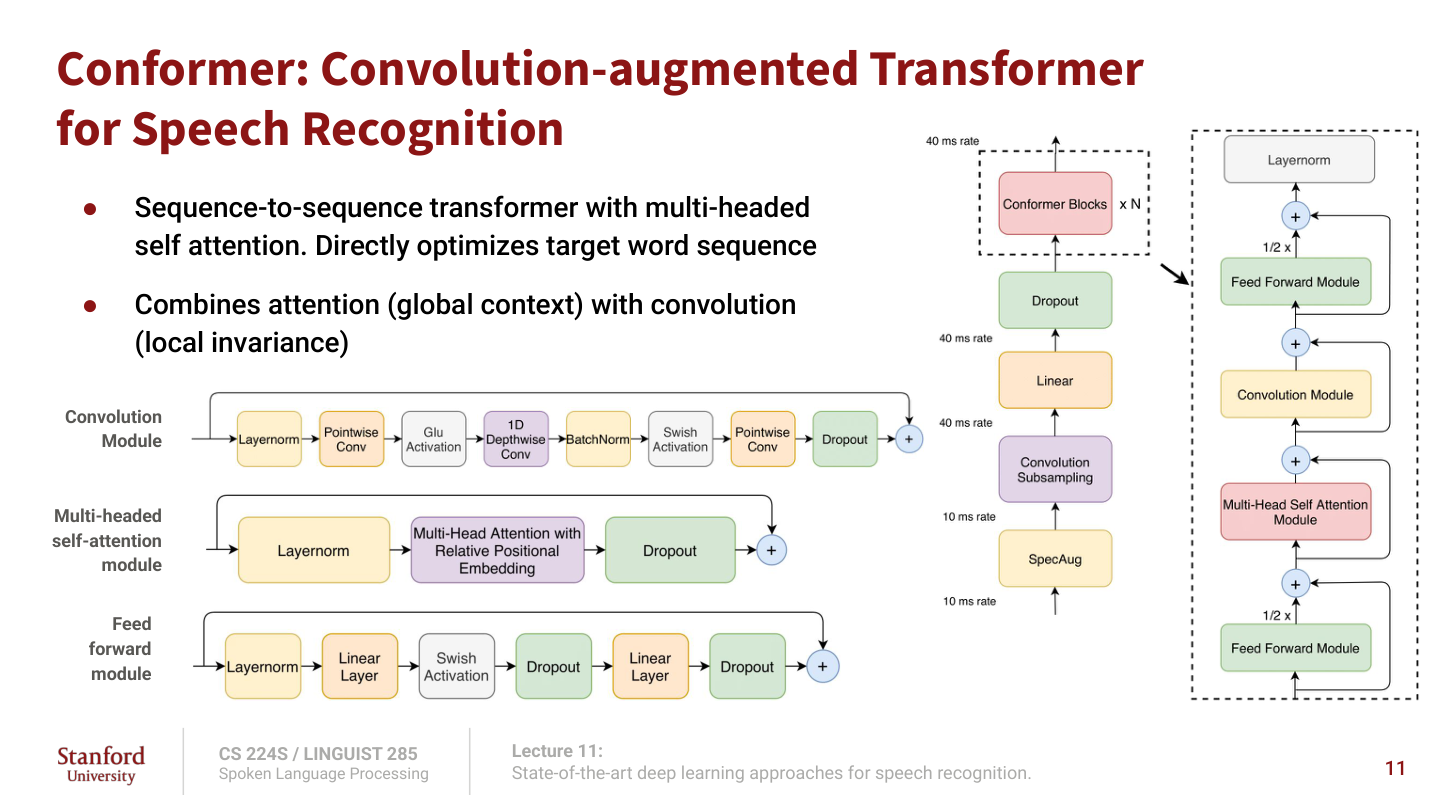
\includegraphics[width=\textwidth,height=0.92\textheight,keepaspectratio]{assets/New-Lecture-STT/cs224s_lec11_slide_11.png}
% \end{frame}

% --- Stanford CS224S lec11, slide 13 ---
\begin{frame}{The convolution block has a\newline greatest effect on performance}
  \begin{columns}[c]
    \begin{column}{0.51\textwidth}
      \vspace{-1.2em}
      \begin{itemize}
        \item From ablation experiment of the paper, \textbf{removing unique features and moving towards a vanilla Transformer block} was tested.
        \item All ablation study results are evaluated without external LM.
      \end{itemize}
      \vspace{1.4em}
      \textcolor{KAred}{\textbf{The convolution block has the greatest effect on performance.}}
    \end{column}
    \begin{column}{0.47\textwidth}
      \centering
      \\[0.3em]
      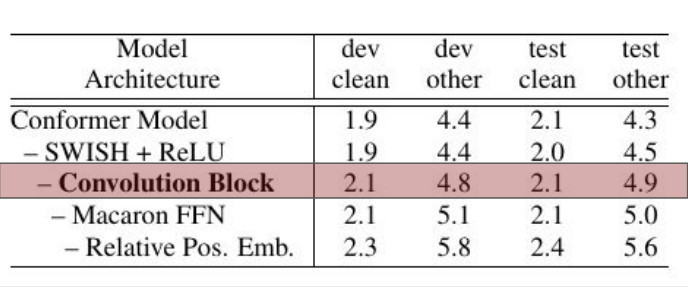
\includegraphics[width=\textwidth,height=0.92\textheight,keepaspectratio]{assets/New-Lecture-STT/cs224s_lec11_slide_13.png}
      {\scriptsize \textit{Ablation results: Largest WER drop from convolutions.}}
    \end{column}
  \end{columns}
\end{frame}

% --- Stanford CS224S lec11, slide 18 ---
\begin{frame}{State-of-the-art ASR: Whisper}
  \centering
  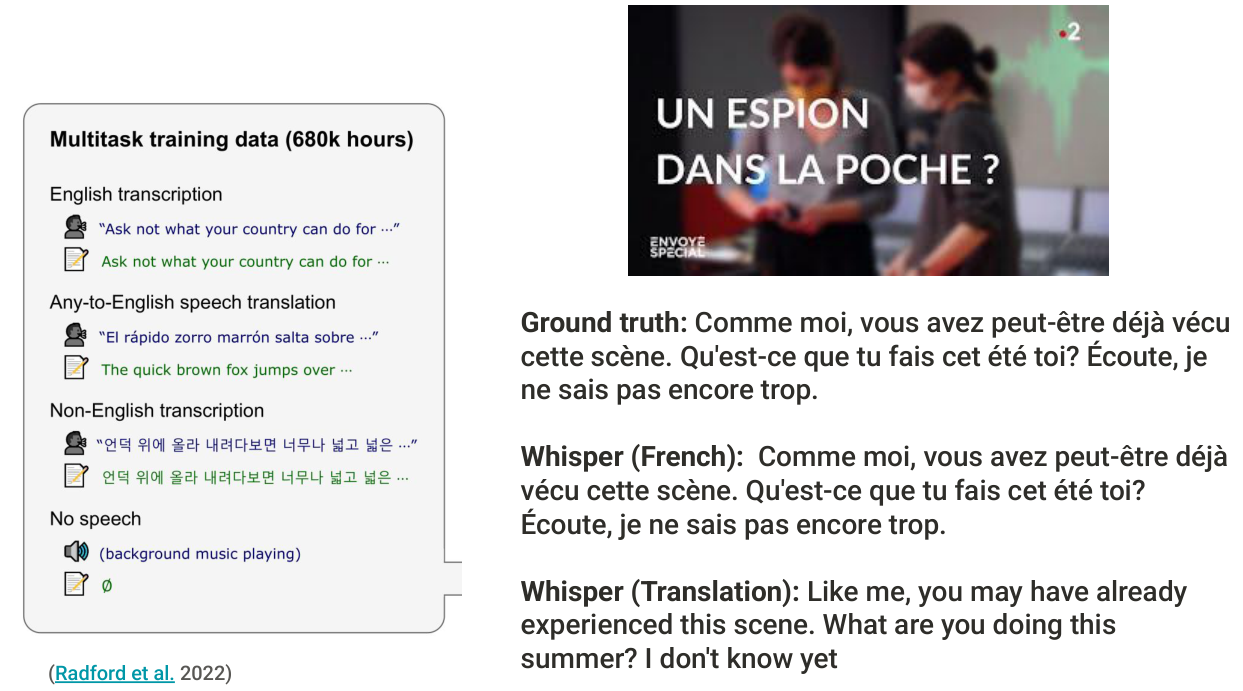
\includegraphics[width=\textwidth,height=0.92\textheight,keepaspectratio]{assets/New-Lecture-STT/cs224s_lec11_slide_18.png}
\end{frame}

% --- Stanford CS224S lec11, slide 20 ---
\begin{frame}{Whisper: How does it perform a variety of tasks accurately?}
  \centering
  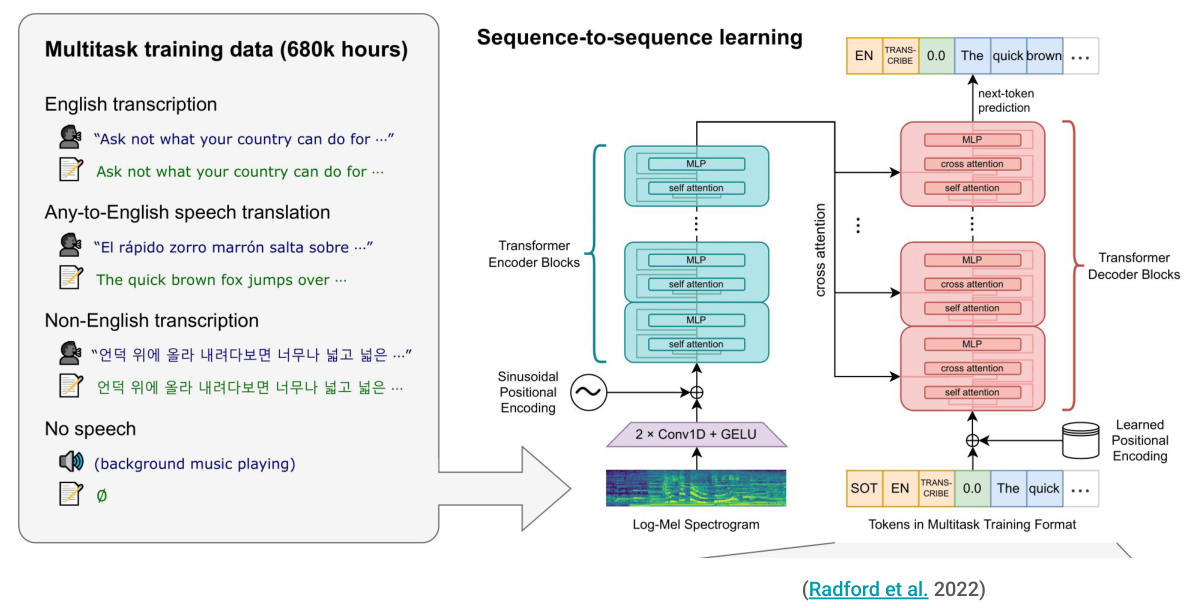
\includegraphics[width=\textwidth,height=0.92\textheight,keepaspectratio]{assets/New-Lecture-STT/cs224s_lec11_slide_20.png}
\end{frame}

% --- Stanford CS224S lec11, slide 21 ---
\begin{frame}{Whisper: encoder--decoder architecture}
  \centering
  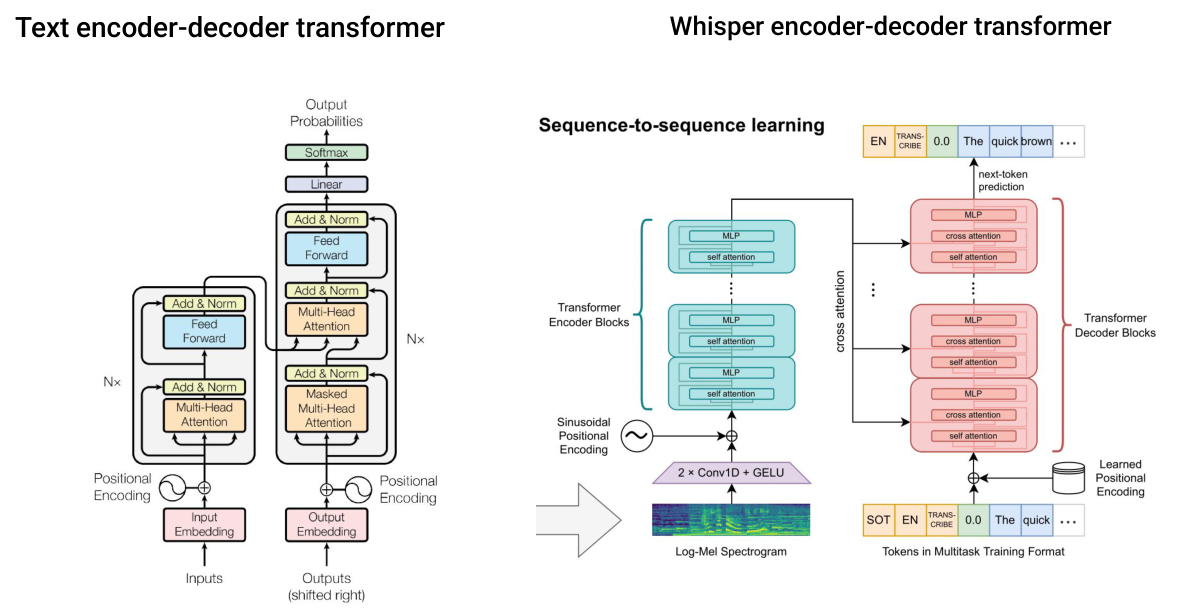
\includegraphics[width=\textwidth,height=0.92\textheight,keepaspectratio]{assets/New-Lecture-STT/cs224s_lec11_slide_21.png}
\end{frame}

% --- Stanford CS224S lec11, slide 22 ---
\begin{frame}{Whisper encoder}
  \begin{columns}[c]
    \begin{column}{0.41\textwidth}
      \raggedright
      \textbf{\textcolor{KAred}{Whisper encoder:}\\ transformer encoder}
      \begin{itemize}
        \item Encoder input: log-mel spectrogram and two convolutional layers
        \item Positional embeddings
        \item Standard transformer blocks depending on model size
      \end{itemize}
      \vspace{1.2em}
      {\scriptsize\textcolor{gray}{CS 224S / LINGUIST 285\\
      Lecture 11: State-of-the-art deep learning approaches for speech recognition.}}
    \end{column}
    \begin{column}{0.58\textwidth}
      \centering
      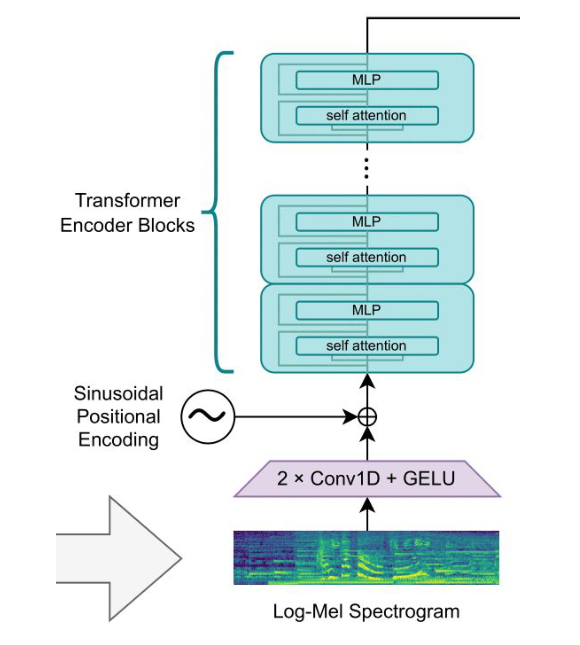
\includegraphics[width=\textwidth,keepaspectratio]{assets/New-Lecture-STT/cs224s_lec11_slide_22.png}
    \end{column}
  \end{columns}
\end{frame}

% --- Stanford CS224S lec11, slide 23 ---
\begin{frame}{Whisper decoder: autoregressive transformer decoder}
  \begin{columns}[c]
    \begin{column}{0.48\textwidth}
      \raggedright
      \textbf{\textcolor{KAred}{Whisper decoder:} autoregressive transformer decoder}
      \begin{itemize}
        \item \textbf{GPT-2 style} model: no more CTC loss.
        \item Decodes using \textbf{auto-regressive prediction}—each token depends on previous (\texttt{text} prediction).
        \item \textbf{Cross-attention:} To encoded audio representation from encoder.
        \item \textbf{Custom vocabulary and tags:}
        \begin{itemize}
            \item Language tags: \texttt{<en>}, \texttt{<fr>}, etc.
            \item Task tags: \texttt{<transcribe>}, \texttt{<translate>}
            \item \textbf{Timestamps}
            \item Speech tags: \texttt{<nospeech>}
        \end{itemize}
      \end{itemize}
    \end{column}
    \begin{column}{0.51\textwidth}
      \centering
      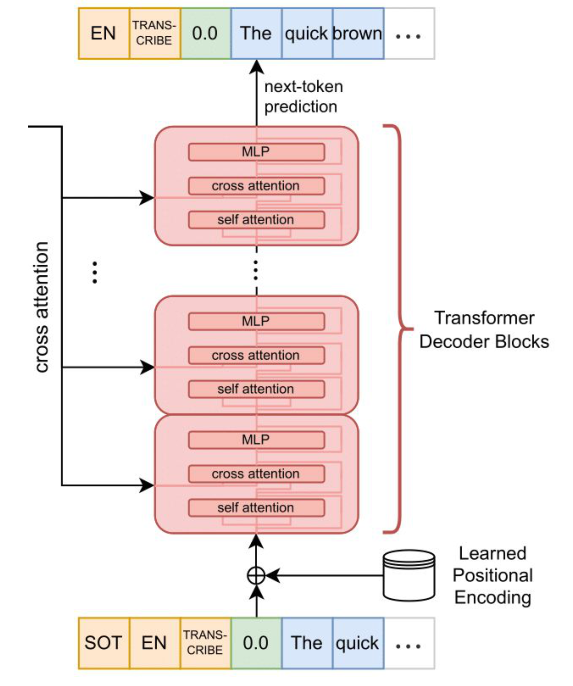
\includegraphics[width=\textwidth,height=0.92\textheight,keepaspectratio]{assets/New-Lecture-STT/cs224s_lec11_slide_23.png}
    \end{column}
  \end{columns}
\end{frame}

% --- Stanford CS224S lec11, slide 30 ---
\begin{frame}{Whisper handles long-form transcription}
  \begin{columns}[T]
    \begin{column}{0.40\textwidth}
      \textbf{Whisper handles long-form transcription}
      \begin{itemize}
        \item Whisper only takes 30 seconds of speech at a time
        \item \textbf{Timestamp tokens} are used to determine when to shift the window
        \item Text from the previous window is provided with transcribing current window
        \item Voice activity detection using \texttt{\textless{}nospeech\textgreater{}} tag
      \end{itemize}
    \end{column}
    \begin{column}{0.60\textwidth}
      \centering
      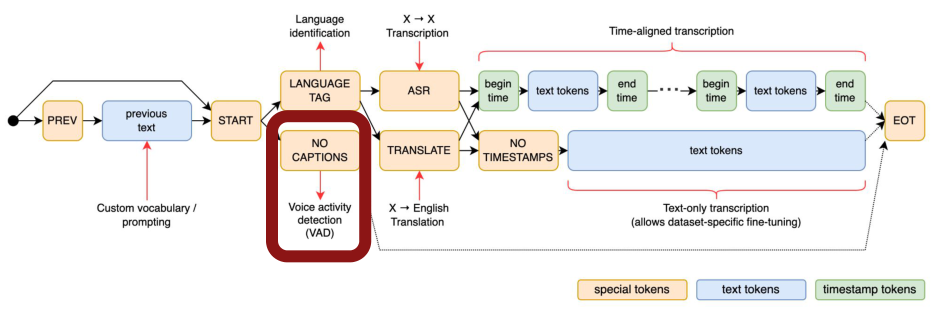
\includegraphics[width=\textwidth,keepaspectratio]{assets/New-Lecture-STT/cs224s_lec11_slide_30.png}
    \end{column}
  \end{columns}
\end{frame}

% --- Stanford CS224S lec11, slide 34 ---
\begin{frame}{Whisper's automatic speech translation performance}
  \begin{columns}[T]
    \begin{column}{0.48\textwidth}
    \centering
    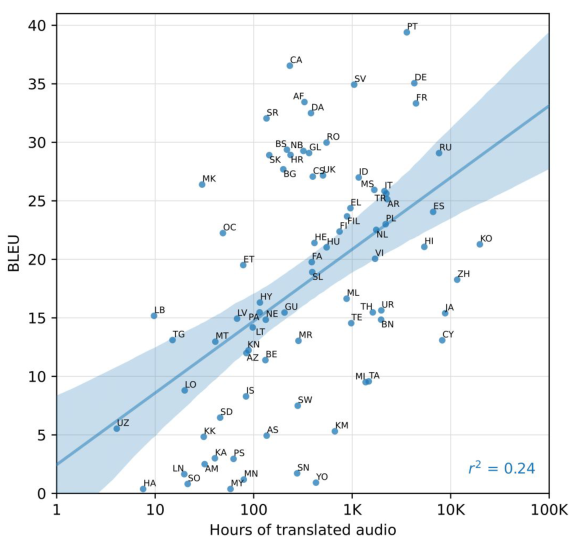
\includegraphics[width=\textwidth,keepaspectratio]{assets/New-Lecture-STT/cs224s_lec11_slide_34.png}
    \end{column}
    \begin{column}{0.50\textwidth}
      \textbf{Speech translation performance on FLEURS dataset (higher is better)}
      \begin{itemize}
        \item Translation performance is better on average after the 100 hours of training data mark.
        \item Amount of training data isn’t as correlated with translation performance as it is with transcription performance.
        \item Although possible, speech translation is likely to only be reliable for high resource languages.
      \end{itemize}
    \end{column}
  \end{columns}
\end{frame}
